% ---------------------------------------------------------------
%  IEEE conference-format source, generated from IAKM_PAPER_V7_DRAFT.md
%  Build:  pdflatex IAKM_PAPER_V7_IEEE  (run twice to resolve \ref)
% ---------------------------------------------------------------
\documentclass[conference]{IEEEtran}
\IEEEoverridecommandlockouts

\usepackage{cite}
\usepackage{amsmath,amssymb}
\usepackage{graphicx}
\usepackage{stfloats}   % lets full-width floats sit at the bottom of a column too
\usepackage{array}

% This paper runs 11 double-column floats. LaTeX's defaults (2 floats and 70%
% of a page top) back the queue up and strand the last tables after the
% references, so the placement limits are loosened here.
\setcounter{topnumber}{2}
\setcounter{bottomnumber}{1}
\setcounter{totalnumber}{3}
\setcounter{dbltopnumber}{2}
\renewcommand{\topfraction}{0.72}
\renewcommand{\bottomfraction}{0.55}
% textfraction is the guard against all-float pages: every page that carries
% body text must give at least this much of itself to text.
\renewcommand{\textfraction}{0.18}
\renewcommand{\floatpagefraction}{0.80}
\renewcommand{\dbltopfraction}{0.72}
\renewcommand{\dblfloatpagefraction}{0.80}
\usepackage{tabularx}
\usepackage[hidelinks]{hyperref}
\usepackage{url}

% ragged-right X columns keep long prose cells from over-stretching
\renewcommand{\tabularxcolumn}[1]{>{\raggedright\arraybackslash}p{#1}}

% W{w} is an X column with a relative width. Per-table weights must sum to the
% number of columns, so a narrow key column buys width for a prose column.
\newcolumntype{W}[1]{>{\hsize=#1\hsize\raggedright\arraybackslash}X}

\begin{document}

\title{Interface-Anchored Knowledge Mapping\\
{\large A Coordinate System for Locating Knowledge-Relevant Metadata in Modular Sociotechnical Systems}}

\author{\IEEEauthorblockN{Elizabeth Osborn}
\IEEEauthorblockA{Pomona, California\\
lizocontactinfo@gmail.com}}

\maketitle

\begin{abstract}
Knowledge loss in modular sociotechnical systems becomes unrecoverable when the conditions that made knowledge usable disappear before they are captured. Documentation, version history, organizational records, meetings and chats, direct observation, dependency models, and telemetry each preserve a partial view, but they do not produce a shared digital map that names the connection between a person and the part of the system they understand, links that connection to sources, and keeps records comparable across collections. 

Interface-Anchored Knowledge Mapping (IAKM) is a digital mapping system and methodology for locating knowledge-relevant metadata in relation to system components and interface relations. It does not seek to store the knowledge itself. Its coordinate system defines the smallest addressable unit as a five-element tuple: governing field, domain, interface layer, component, and knower. Interface layers are binding-relative, so the analytical lens is recorded inside the address, while structural location remains distinct from both the metadata capture point and the carrier in which the knowledge persists. 

Preemptive decomposition supplies candidate structural locations, and ordinary digital work artifacts supply the observational opening. AI-assisted analysis can examine those artifacts at scale while work is still unfolding, but candidates enter the map only through validation, attached evidence, and human verification. A reference implementation deployed on a distributed university aerospace program produced 121 verified nodes and 24 verified edges in its most recent extraction run, under one binding, with partial coverage. The work is at the collection stage: reproducibility, reviewer agreement, cross-domain validity, and predictive value remain untested, and several of those questions cannot be posed until a corpus exists. 
\end{abstract}

\begin{IEEEkeywords}
Artificial intelligence, design structure matrix, domain analysis, knowledge loss, knowledge management, metadata, modularity, organizational memory, sociotechnical systems, verification.
\end{IEEEkeywords}



\section{The Methodological Problem}\label{sec:1}

Knowledge loss in sociotechnical systems becomes unrecoverable when the conditions that made knowledge usable disappear before they are captured. In rapidly developing technical fields, critical knowledge is often formed during the work itself: debugging, integration, tool adaptation, failure interpretation, and design decisions made under pressure. Some of that knowledge becomes documentation, code, diagrams, test records, or procedures. Much of it remains with people: the professor who remembers why a laboratory method changed, the senior student who knows why a subsystem behaves strangely, the engineer who knows why an interface was built a certain way, or the technician who can recognize a failure pattern before it appears in a formal report.

When those people leave, the artifacts may remain while the conditions that made them intelligible disappear. A repository can preserve what was committed without preserving why it was written that way. A document can preserve a procedure after the tools, dependencies, assumptions, or design context that made it valid have changed. An organization can preserve roles without preserving the expertise that once made those roles functional. The contextual meaning that surrounds each artifact degrades, making it more difficult for new cohorts to integrate.

As development accelerates, emerging-technology methods are used and revised simultaneously, tools are often obsolete immediately after they are used, and experimental workflows are patched or abandoned before anyone has time to convert what was learned into durable institutional memory. The result is not merely incomplete documentation. It is a system that remains physically intact, digitally archived, and organizationally staffed while becoming difficult or impossible to understand.

The methodological problem is therefore to make knowledge loss observable before it becomes unrecoverable. Doing that requires a record that locates knowledge-relevant metadata in relation to the system: who appears to know what, what component it concerns, what evidence supports the claim, and where the knowledge may still be recoverable.

\section{What Existing Methods Make Visible, and Why Loss Persists}\label{sec:2}

Existing methods already preserve parts of this problem. The question is whether any of them also preserves the relation needed for recovery: who appears connected to knowledge about a specific part of the system, on what evidence, and in a form that can be checked later.

Table~\ref{tab:methods} compares what each method makes visible and what remains outside its record. Fig.~\ref{fig:timing-coverage} places the same methods on two axes that matter for recovery: when the observation happens, and how much of the program it reaches.

\begin{table*}[!tb]
\caption{What existing methods make visible, and what remains outside their records.}
\label{tab:methods}
\centering
\scriptsize
\begin{tabularx}{\textwidth}{XXX}
\hline
\textbf{Method or record type} & \textbf{What it makes visible} & \textbf{What it still misses} \\
\hline
Documentation & Procedures, explanations, requirements, and design descriptions & Tacit judgment, changing assumptions, tool drift, and context that was not written down \\
Repositories and version history & Code, authorship traces, sequencing, and change over time & Why a change mattered, who still understands it, and whether its rationale remains recoverable \\
Organizational records & People, roles, assignments, authority, and responsibility & Component-specific knowledge and the conditions under which a person came to know \\
Meetings, chats, and recorded calls & Discussion, coordination, rationale, questions, informal decisions, and explanations as work unfolds & Stable structural address, later recoverability, and whether the knowledge persists outside the conversation \\
Direct observation of work in progress & Knowledge as it is used, seen at the site of the work & Coverage across teams that are distributed and working at once \\
Systems engineering, DSM, MBSE, and dependency models & Components, interfaces, couplings, and technical structure & Which people understand which parts, and on what grounds \\
Telemetry and logs & Runtime behavior, failures, and operational traces & The human interpretive knowledge needed to explain why behavior occurred \\
AI-assisted artifact analysis & Large-scale candidate extraction from available artifacts while work is ongoing & Scientific validity, unless constrained by address, evidence, metadata, and verification \\
\hline
\end{tabularx}
\end{table*}

A digital mapping system for knowledge loss depends on several claims that are already established in other literatures: that systems can be decomposed into components and interfaces, that knowledge can be lost when people and practices change, and that the field of analysis shapes what becomes visible. Table~\ref{tab:literature} identifies which part of that foundation each literature supplies.

\begin{table*}[!tb]
\caption{Established results the methodology builds on, and what it takes from each.}
\label{tab:literature}
\centering
\scriptsize
\begin{tabularx}{\textwidth}{W{1.3}W{0.35}W{1.35}}
\hline
\textbf{What the literature establishes} & \textbf{Source} & \textbf{What the methodology takes from it} \\
\hline
Systems decompose into subsystems whose internal interactions exceed those between them & \cite{simon1962} & Components are identifiable enough to anchor an address \\
Interfaces carry types and differential magnitude, so a pair is described by a vector & \cite{pimmler1994} & Coupling strength is recorded per layer, never as one number \\
The design structure matrix tradition has extended that representation across lineages & \cite{browning2016} & The representation can be adopted rather than argued for \\
Organizations accumulate knowledge through experience and lose it over time & \cite{argote1999} & The loss is real and has been measured \\
Departures can reduce recoverable expertise, though severity by structural position is unsettled & \cite{galan2023} & A recovery record must capture position and knower before the question can be posed \\
Knowledge can be associated with activity and position, but observing it requires presence & \cite{lave1991,hutchins1995} & Location was reached once, by a method that does not scale \\
The field under which a system is examined governs what becomes visible within it & \cite{hjorland1995,hjorland2002} & The field and domain of analysis have to be declared inside the record \\
\hline
\end{tabularx}
\end{table*}

Across the methods surveyed here, the missing element is a shared way to record the connection between a person and the part of the system they understand. These methods preserve useful evidence, but they do not produce a digital map that names that connection, links it to sources, and keeps it comparable across collections.


\begin{figure*}[!tb]
\centering
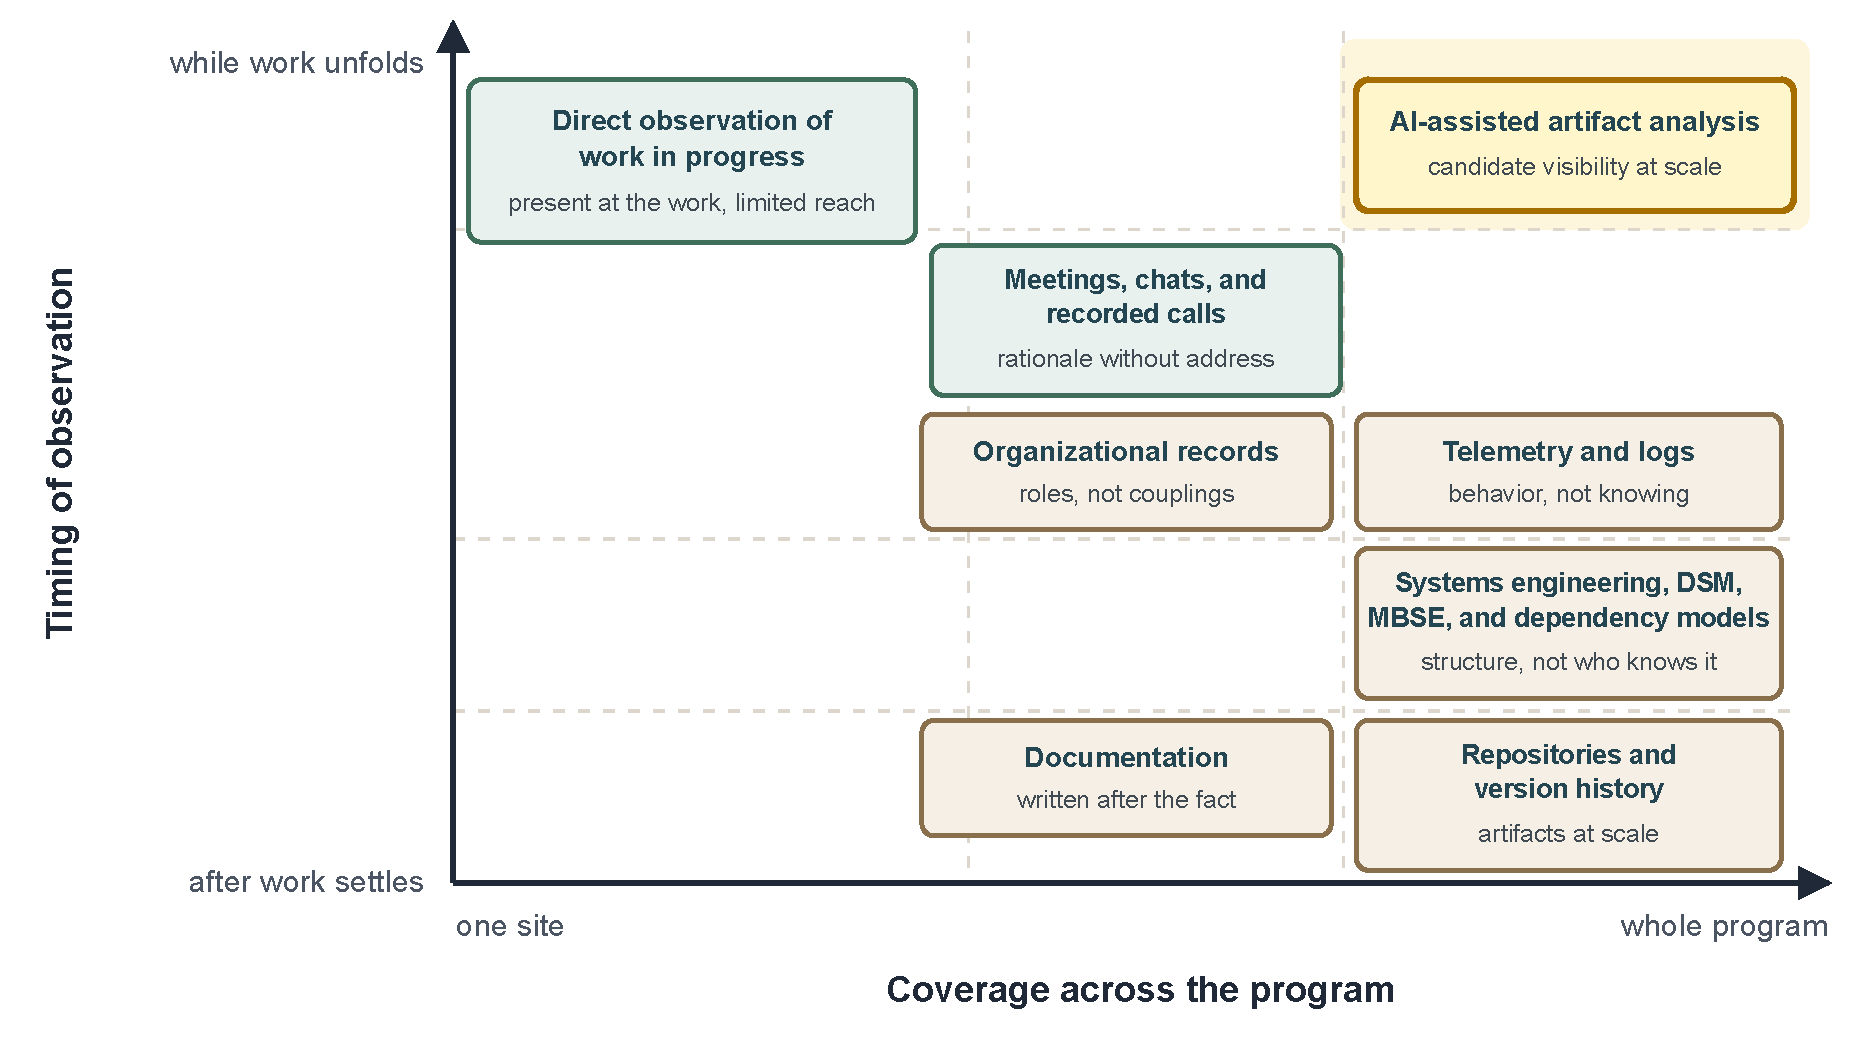
\includegraphics[width=0.70\textwidth]{fig2_timing_coverage_plane_print.pdf}
\caption{Existing methods plotted by timing of observation and coverage across the program. Methods that observe while work unfolds reach one site at a time. Methods that reach the whole program observe after the work has settled. Only AI-assisted artifact analysis reaches the upper right, observing while work is still unfolding and across the whole program, and it reaches that region without supplying the constraint that makes the observations verifiable.}
\label{fig:timing-coverage}
\end{figure*}


\section{Preemptive Decomposition}\label{sec:3}

A mapping system for knowledge loss requires the system to be decomposed before the loss occurs. Components, couplings, boundaries, and interfaces must be identifiable while the people, artifacts, practices, and traces that carry recoverable knowledge are still present.

The decomposition comes from a structural model of the sociotechnical system rather than from the knowledge record itself. That role can be filled by nearly decomposable architecture, which treats the system as a molecular structure: bond strengths between elements differ by orders of magnitude, so modules are defined by relatively tighter internal bonds and looser relations across boundaries [1]. Couplings are the relations between parts, typically stronger inside a module than across its boundary. Interfaces occur where parts connect, within modules as well as across module boundaries. Sustaining mechanisms are the formal or informal structures that keep an interface working, such as a role, tool, protocol, or shared repository. The first three of these units, module, coupling, and interface, are inherited from systems and modularity literature. A sustaining mechanism field is added because a sociotechnical interface is not fully described by the fact that a connection exists; the record also needs to state what, if anything, keeps that connection usable.

Preemptive decomposition matters because it gives the later map places to look. Once components and interfaces are identifiable, knowledge-relevant metadata can be sought at the relations where people, artifacts, tools, practices, and system parts meet. At the present collection stage, interface characterization guides search by suggesting what kinds of evidence may be recoverable. It remains a heuristic rather than a proof rule until repeated collections show whether those interface characteristics correspond reliably to recoverable metadata.

Preemptive decomposition identifies candidate structural locations; the record-producing procedure in Section~\ref{sec:6} depends on those locations before an address can be anchored.

\section{Digital Interfaces as the AI Seam}\label{sec:4}

The new observational opening is digital. Modern technical work produces repositories, issues, reviews, documents, logs, chats, meeting records, workflow traces, and other artifacts as part of ordinary activity. These records do not preserve knowledge completely, but they often preserve metadata about where knowledge was used, who was involved, what component was affected, what decision or failure prompted action, and where recovery may still be possible.

Artificial intelligence changes the scale and timing of that observation. Earlier methods either observe knowledge-rich activity while it is happening but only locally, or preserve records at scale after the work has settled. AI-assisted analysis can examine large bodies of ordinary work artifacts while the work is still unfolding. That allows candidate interface relations to be identified before the people and traces that make verification possible have disappeared.

AI identifies candidate observations from digital traces. A methodology is still required to structure those candidates, attach evidence, distinguish metadata from knowledge content, and verify which records enter the map.

Interface-Anchored Knowledge Mapping (IAKM) is a digital mapping system that uses artificial intelligence to locate knowledge-relevant metadata about a physical system. It does not claim to capture the knowledge itself. It produces structured records about what appears to be known, who is implicated in that knowing, what component of the system the knowledge concerns, where the relevant interface relation is exposed, what evidence supports the observation, how the knowledge is grounded, and where the knowledge remains recoverable.

The methodology of IAKM specifies how those observations are decomposed, addressed, checked, and preserved. Its coordinate system gives each verified record a structural address, so that records can be found again, compared across collections, audited against evidence, and accumulated into a corpus.

The methodology is specified for modular sociotechnical systems in which components can be identified, ordinary work produces artifacts, and a governing field can be declared. It is not specified for systems without identifiable components, for knowledge unrelated to any component, or for settings where no artifact record exists.

The reference implementation appears only as evidence that portions of the methodology were exercised in software, and to state what was and was not demonstrated.

\section{The Recovery Record and Coordinate System}\label{sec:5}

IAKM does not need to store the knowledge itself. No copy of it, no summary of it, and no permanent access to it is required once a verified record has adequate provenance. That is the part that runs against ordinary intuition.

Preservation is usually taken to mean capture, so knowledge that cannot be written down has often been treated as already lost. A component that depends on one person is nonetheless a fact about the system, and that fact can be established without anyone writing down what the person knows. The connection is observable whether or not the content is.

The record is one of metadata rather than content. It preserves enough to locate, verify, and revisit a knowledge-relevant relation after people, tools, documents, or organizational roles have changed.

Three senses of location run together in ordinary speech, and the methodology keeps them apart because each does different work. Table~\ref{tab:senses} states the distinction and Fig.~\ref{fig:three-senses} shows how the three relate.

\begin{table*}[!tb]
\caption{Three senses of location kept distinct by the methodology.}
\label{tab:senses}
\centering
\scriptsize
\begin{tabularx}{\textwidth}{XXX}
\hline
\textbf{Sense of location} & \textbf{What is located} & \textbf{Function in the methodology} \\
\hline
Structural location & The interface relation between a knower and a component, under a declared field, domain, and layer & Gives the record an address: the relation can be found again, compared, queried, and joined with other records \\
Metadata capture point & The place in the available evidence where descriptors of the relation are observed & Shows where the methodology recovered evidence about the relation, without implying that the knowledge itself resides there \\
Carrier location & The person, artifact, instrument, model, practice, or community in which the knowledge itself appears to persist & Shows where recovery, transfer, preservation, or loss would take place \\
\hline
\end{tabularx}
\end{table*}


\begin{figure*}[!t]
\centering
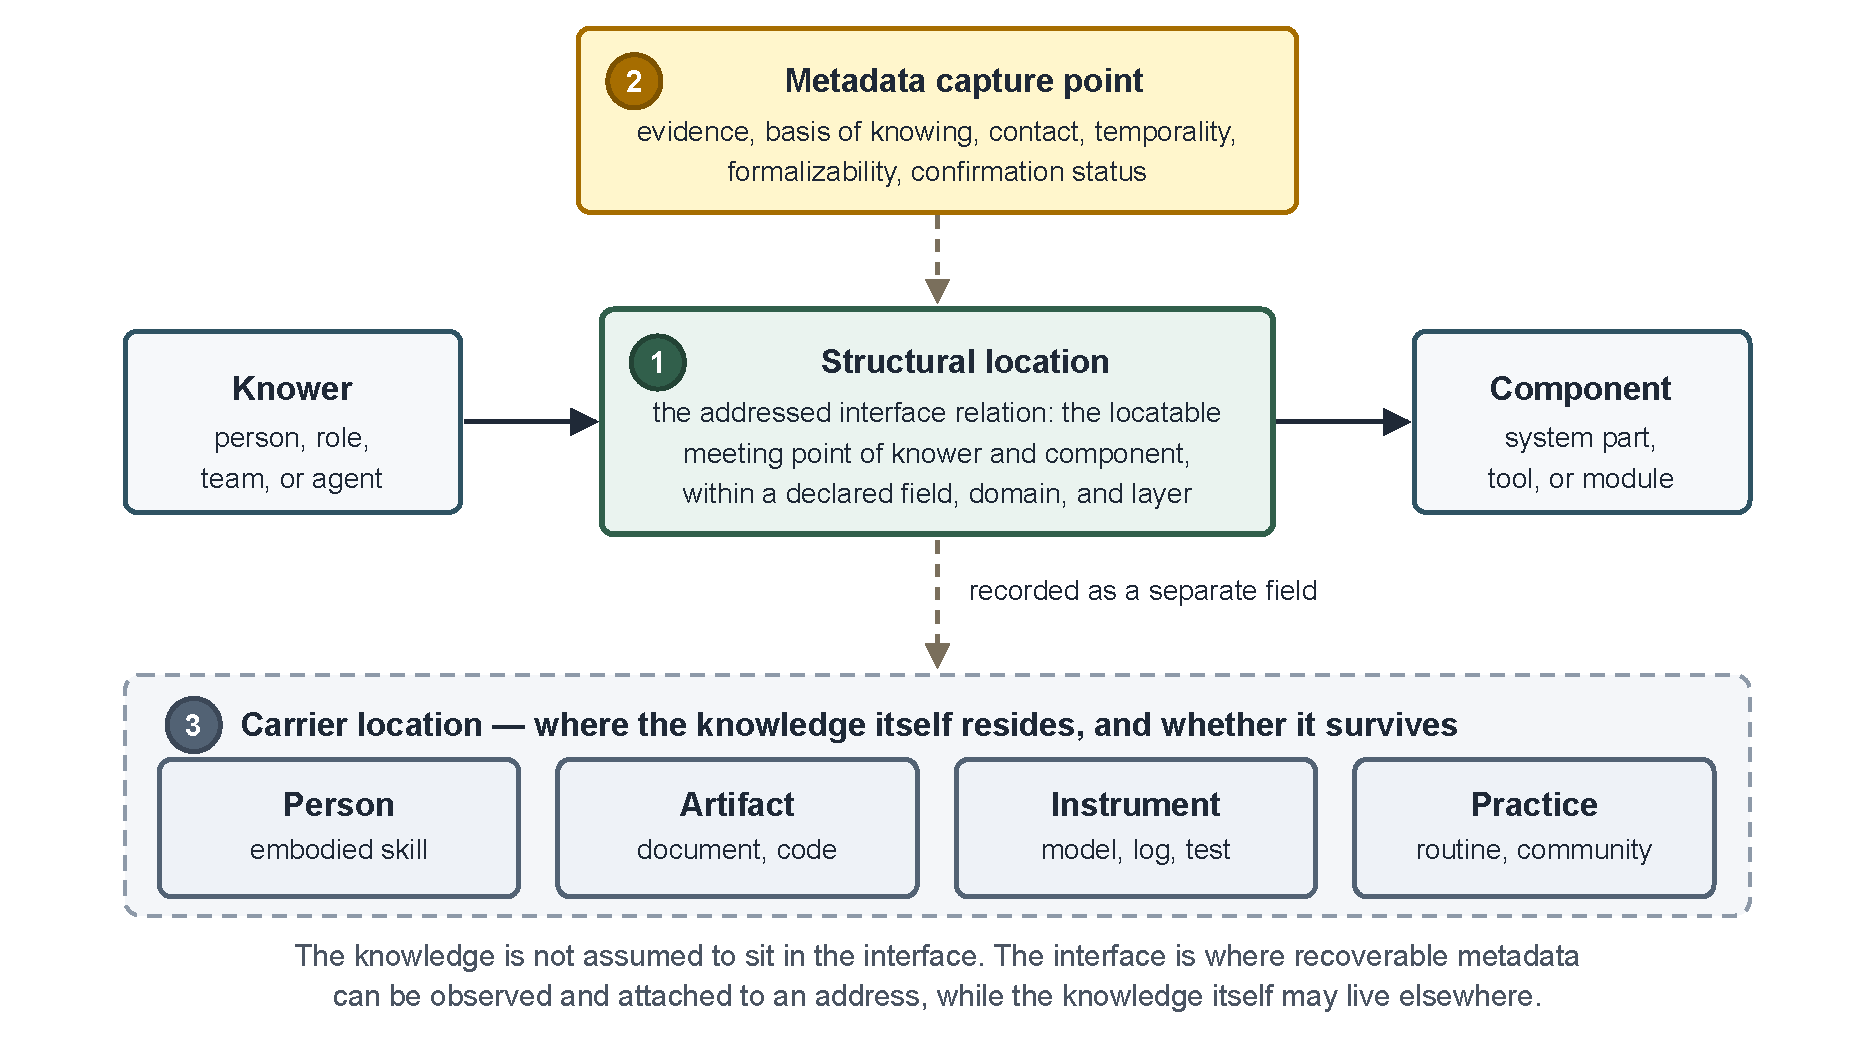
\includegraphics[width=0.86\textwidth]{fig1_three_senses_of_location_print.pdf}
\caption{The three senses of location. The structural location is the addressed interface relation between knower and component under a declared field, domain, and layer. The metadata capture point is where evidence about that relation was observed. The carrier location, recorded as a separate field, is where the knowledge itself appears to persist. The knowledge is not assumed to sit in the interface.}
\label{fig:three-senses}
\end{figure*}


The technician who knows by feel when a connector has seated is the case that makes the separation necessary. The content of what that person knows is not in the digital record and may never be. The relation is addressed because the component, knower, field, domain, and interface layer can be named. The capture point may be thin: perhaps a maintenance note, a repeated repair pattern, or a test anomaly. The carrier is recorded as the person, and the record therefore states that a specific component depends on knowledge held in one body and nowhere else. That is a structural condition the record can state, produced without capturing the knowledge itself.

A digital map requires stable addresses. The coordinate system supplies them for verified records. IAKM anchors the record to the relation between a knower and a component, rather than to the record itself or to only one end of the relation.

The smallest addressable unit is one interface layer, under one declared field and domain, between one component and one knower:

\begin{equation}
A = (T_{1},\, T_{2},\, T_{3},\, C,\, K)
\end{equation}

Table~\ref{tab:address} defines each element.

\begin{table*}[!tb]
\caption{Elements of the address, and why the record requires each.}
\label{tab:address}
\centering
\scriptsize
\begin{tabularx}{\textwidth}{W{0.4}W{1.45}W{1.15}}
\hline
\textbf{Element} & \textbf{Meaning} & \textbf{Why the record requires it} \\
\hline
T1 & Governing field: the body of methods, vocabulary, and standards of evidence used as the analytical lens & Fixes the standards of evidence under which the relation is claimed \\
T2 & Domain: the subject area into which the governing field reaches & One field reaches several subject areas, and which one is in play has to be fixed \\
T3 & Interface layer: the structural connection layer exposed by the declared field and domain & Locates where the relation between knower and component is exposed \\
C & Component anchor: the part of the system the metadata concerns & Identifies what part of the system the knowledge concerns \\
K & Knower anchor: the person whose knowledge, role, authorship, observation, or responsibility is implicated & Identifies whose knowledge is implicated \\
\hline
\end{tabularx}
\end{table*}

A binding is the declared pair (T1, T2): the governing field and the domain to which it is applied. The binding determines which interface layers are visible. A software-architecture binding and a hardware-integration binding may expose different layers for the same person-component pair. They can still be joined through shared component and knower anchors. There is therefore no universal set of interface layers, no fixed count, and no canonical ordering across systems.

Nothing else belongs in the address. The descriptors below attach to an address without forming part of one, because none of them tells two addresses apart and several can change while the relation stays where it is. Holding that line prevents the address from being read as a container for knowledge content.

Table~\ref{tab:descriptors} lists the descriptors that attach to an address without becoming part of it.

\begin{table*}[!tb]
\caption{Descriptors attached to an address, and why each is not part of address identity.}
\label{tab:descriptors}
\centering
\scriptsize
\begin{tabularx}{\textwidth}{W{0.78}W{1.17}W{1.05}}
\hline
\textbf{Attached descriptor} & \textbf{What it records} & \textbf{Why it is not part of the address} \\
\hline
Interaction type & What kind of relation crosses the interface & Relations of different kinds can be exposed at one address, so type does not tell two addresses apart \\
Sustaining mechanism & Who or what keeps that relation working & A mechanism can be added or removed while the relation stays at the same address \\
Coupling strength & The strength of that structural connection & A value that moves over time cannot be part of what makes two records the same \\
Evidence and lineage & The source material the observation rests on & Two analysts can reach one address from different evidence \\
Epistemic metadata & How the knowledge was grounded & It describes the knowing rather than the position the knowing occupies \\
Carrier or persistence location & Where the knowledge itself appears to persist & The carrier can change while the structural relation is unchanged \\
Confirmation status & Whether the record has been admitted to the verified map & Status changes through the procedure, so it is attached to the address rather than part of address identity \\
\hline
\end{tabularx}
\end{table*}

Type and strength are what the design structure matrix tradition already records about an interface [2]. Sustaining mechanism adds a separate descriptor: what, if anything, keeps the relation usable.

Address identity is strict, and partial agreement is still informative. Two records refer to the same address only when all five elements match, which is what allows independent records of one system to be differenced. Records produced under different bindings still join through their shared component and knower anchors, without collapsing the layers each binding exposes. Holding a component fixed while varying the knower makes visible how many knowers are named at that component.

A component at which exactly one verified address names a knower is a structural condition of the record, and not by itself a prediction that knowledge will be lost.

Several constraints follow from the coordinate system. The address must remain exactly A = (T1, T2, T3, C, K), because adding metadata fields to the tuple would make address identity unstable. Interface layers must remain binding-relative, because a layer visible under one field and domain may not exist under another. Evidence and lineage must remain attached, because later readers must be able to check why a record was admitted. Structural location and carrier location must remain distinct, because the relation being mapped is not the place where the knowledge itself necessarily persists.

An implementation instantiates IAKM only if it preserves these constraints. The coordinate system defines what a record must preserve; the next step is the procedure that determines how candidate records are produced, checked, and admitted to the verified map.

\section{Procedure for Producing Verified Records}\label{sec:6}

The procedure begins from the decomposition set out in Section~\ref{sec:3}, which IAKM presumes rather than derives, and which must be in place before an address can be anchored. With that decomposition available, the IAKM methodology produces verified map records through candidate extraction, validation, and human verification. Computation over the verified record comes afterward.

Table~\ref{tab:procedure} gives the procedure step by step.

\begin{table*}[!tb]
\caption{Procedure for producing verified records.}
\label{tab:procedure}
\centering
\scriptsize
\begin{tabularx}{\textwidth}{W{0.5}W{1.35}W{1.15}}
\hline
\textbf{Step} & \textbf{What is done} & \textbf{What it yields} \\
\hline
Represent & Identify components and structural couplings & Anchors for C \\
Select & Declare the governing field and domain & The binding, (T1, T2) \\
Configure & Translate system structure into the layers that binding exposes & The layer set for T3 \\
Ingest & Read artifacts as ordinary work already produces them & Source material, unaltered \\
Identify & Locate five-element addresses with metadata attached & Candidate records \\
Validate & Check lineage, duplicates, schema, identities, layer validity & Validated candidates \\
Verify & A person with standing dispositions each candidate & Approved, corrected, rejected, or duplicate \\
Admit & Promote verified records only & The map \\
\hline
\end{tabularx}
\end{table*}

Candidate records remain separate from verified records throughout, because extraction is not confirmation.

During collection, metadata is recovered from available evidence about addressed interface relations, and what IAKM preserves is the verified recovery record rather than the source it was recovered from. Teams are not asked to author documentation for the map; the ingest step reads repositories, issues, reviews, documents, logs, wikis, contracts, and meeting records as they already exist. Each candidate carries the five-element address with the Section~\ref{sec:5} descriptors attached and the evidence held as a source snapshot. Of the four dispositions, the two that alter or exclude a candidate require a recorded reason, so that a later reader can distinguish a rejected claim from one never made. Queries, exports, gradients, composition, and change analysis operate on the verified store by default.

Verification has stated criteria, and they are what a reviewer with standing is checking. First, that the address is correctly located, meaning the component, knower, field, domain, and layer named are the ones the cited evidence supports. Second, that each attached descriptor is supported by that evidence rather than inferred beyond it. Third, that the seven epistemic questions are answered from the same evidence, with an unknown recorded as an unknown rather than left blank. A failed check produces a disposition other than approval, and the recorded reason names which check failed.

Epistemic metadata is recorded against seven named questions rather than as free commentary, each carrying its own recorded fields. The questions ask who knew the relevant knowledge and how close they were to the system; where the knowledge lives now; what must stay connected for it to work; under what conditions it was true; when it stops being reliable; who wrote or taught it and why; and whether it works only while someone keeps doing it. Naming the questions allows two analysts to produce comparable records. They elicit answers rather than scoring them. No threshold, weighting, or score is defined over the answers, and every question concerns what can be recovered from the available evidence about an addressed interface relation and where the knowledge itself appears to persist.

\section{Reference Implementation and Deployment Status}\label{sec:7}

\subsection{Reference Implementation}\label{sec:7-1}

The reference implementation was built to capture knowledge-relevant metadata during rapid, distributed technical development. It used automated extraction, staged review, provenance preservation, and a verified knowledge graph while the work was still unfolding. Here it is treated as one software embodiment of the methodology, showing which parts were exercised, which remained partial, and which implementation requirements became visible during use.

The implementation ingested sources, preserved raw snapshots, extracted candidate records with classification applied at capture, ran automated validation, presented candidates for human review, and promoted approved records into a verified store. Its design boundary separates replaceable extraction infrastructure from the methodology-bearing layers: address structure, metadata, provenance, validation, and verification. Extraction technology is expected to change, and the record structure is what the methodology contributes.

\subsection{Deployment and Run-level Finding}\label{sec:7-2}

The implementation was built and deployed across five universities in a distributed aerospace program whose teams were developing CubeSat missions on a shared open-source hardware platform and a shared open-source modular flight software framework. For tractability, the deployment used one binding, meaning one declared field-and-domain lens, rather than mapping the program under multiple bindings. That binding exposed five interface layers. The available sources reached two of them: documentation and software.

In the most recent extraction run, the agents produced 121 verified nodes and 24 verified edges in the knowledge graph, with 199 candidates pending in the review queue. These figures record what that run extracted, validated, and stored. They are not cumulative totals, evidence of a complete five-element address set, or evidence that the methodology was exercised in full. More material was extracted and validated than was confirmed, which is the expected behavior of a review step that filters candidates rather than passing them through. Coverage was partial, and the record is a sample rather than a census.

The run showed that the implementation could produce structured candidate records from ordinary work artifacts, keep candidate and verified records separate, and promote reviewed records into a verified knowledge graph. The run suggested that some forms of knowledge were more visible in available sources than others. Knowledge already expressed in documents, code, or other artifacts was directly observable. Knowledge held in practice, judgment, or bodily skill was less directly visible, though the structural positions associated with it could sometimes be named. It did not show predictive validity, long-term performance, intervention effects, coupling-strength calibration, reviewer agreement at scale, complete census, or which mapping choices suit other domains.

\subsection{Demonstration Status and Limits}\label{sec:7-3}

The status of each element differs, and collapsing the differences into a single disclaimer would misstate the work in both directions. Table~\ref{tab:status} separates three statuses. Specified means the methodology defines the element. Implemented means the reference implementation included it in software. Demonstrated means the deployment exercised it and left an outcome in the record. No row was measured against an external criterion; Section~\ref{sec:9} describes what such checks would require.

\begin{table}[!t]
\caption{What is specified, implemented, and demonstrated.}
\label{tab:status}
\centering
\scriptsize
\begin{tabularx}{\columnwidth}{Xccc}
\hline
\textbf{Element} & \textbf{Specified} & \textbf{Implemented} & \textbf{Demonstrated} \\
\hline
Five-element address & yes & partial & no \\
Candidate and verified separation & yes & yes & yes \\
Evidence and lineage & yes & yes & partial \\
Explicit unknown as a value & yes & partial & no \\
Epistemic metadata & yes & partial & partial \\
Gradient & yes & no & no \\
Multi-domain composition & yes & no & no \\
Propagation & yes & no & no \\
Census closure & open & no & no \\
\hline
\end{tabularx}
\end{table}

The distinction matters because a feature can be specified by the methodology, implemented in software, or demonstrated in deployment without occupying all three states.

Verification coverage was partial, and the reason belongs in the result. The team dispersed before review at scale was possible, so the lead researcher verified a representative sample rather than the program's engineers verifying every candidate. The methodology admits both arrangements and requires that a study declare which was used. The deployment shows that the review gate operates, not that it was operated at full coverage.

The deployment did not evaluate sustained use. It did not measure operator workload, reviewer agreement, cohort transfer, or predictive validity. Those questions require multiple operators, repeated review cycles, and later beneficiaries using the verified library.

\subsection{Requirements Observed During Use}\label{sec:7-4}

Four implementation failures during use produced requirements for future implementations of this kind:

\begin{enumerate}
  \item Completeness must be checked against stored counts, not assumed from a clean exit.
  \item Classification must occur when a relationship is first captured, because type cannot be reliably reconstructed afterward.
  \item Invocation limits must not silently drop validated records.
  \item Cross-source identity conflicts must be detected and resolved during verification.
\end{enumerate}

These are implementation requirements, not additional methodology rules.

The partial deployment is enough to show that verified records can be produced, but not enough to establish every use available to a mature map. The next section separates those uses from the evidence needed to validate them.

\section{Uses of Verified Map Records}\label{sec:8}

The implementation produced only a partial verified map, but the record structure specifies operations that become available once verified records exist. Verified records can be used immediately for queries and structured review. Other uses require repeated collections or a corpus.

Table~\ref{tab:uses} lists the operations verified records support, and the guardrail on each.

\begin{table*}[!tb]
\caption{Uses of verified map records, with guardrails.}
\label{tab:uses}
\centering
\scriptsize
\begin{tabularx}{\textwidth}{XXXX}
\hline
\textbf{Use} & \textbf{Record basis} & \textbf{What it yields} & \textbf{Guardrail} \\
\hline
Query and retrieval & Verified records under a declared binding & Which records exist at a given component, knower, or layer & Available once verified records exist; results are only as complete as the verified map \\
Knowledge gradient & Verified addresses differing only by layer, at one (T1, T2, C, K) & A vector of layer-specific coupling strengths & Requires enough verified layer records under one binding; not defined across bindings \\
Multi-domain composition & Maps made under different bindings & A join at their shared C and K anchors & Differences across bindings are observations, not errors \\
Change and departure analysis & Verified addresses naming one knower & The components and layers connected to that person & Identifies affected records; does not by itself predict loss \\
Absence and unknown states & Addresses at which something was expected & An explicit unknown, distinct from a blank & Meaningful only where an address and expectation exist \\
Repeated collection & The same sources collected again under the same convention & Change in the records between collections & Requires comparable conventions over time; enables trajectories, not causal claims by itself \\
\hline
\end{tabularx}
\end{table*}

The gradient is a layer profile rather than a single score. That distinction matters because different weak layers point to different preservation actions: a weak documentary layer may call for documentation, while a weak embodied or physical-contact layer may call for demonstration, paired work, or practice. Fig.~\ref{fig:gradient-vector} shows two components whose scalar summaries are identical and whose layer profiles call for opposite interventions. Any scalar reduction, propagation model, or predictive use of the gradient remains unvalidated until tested in a particular study.


\begin{figure*}[!t]
\centering
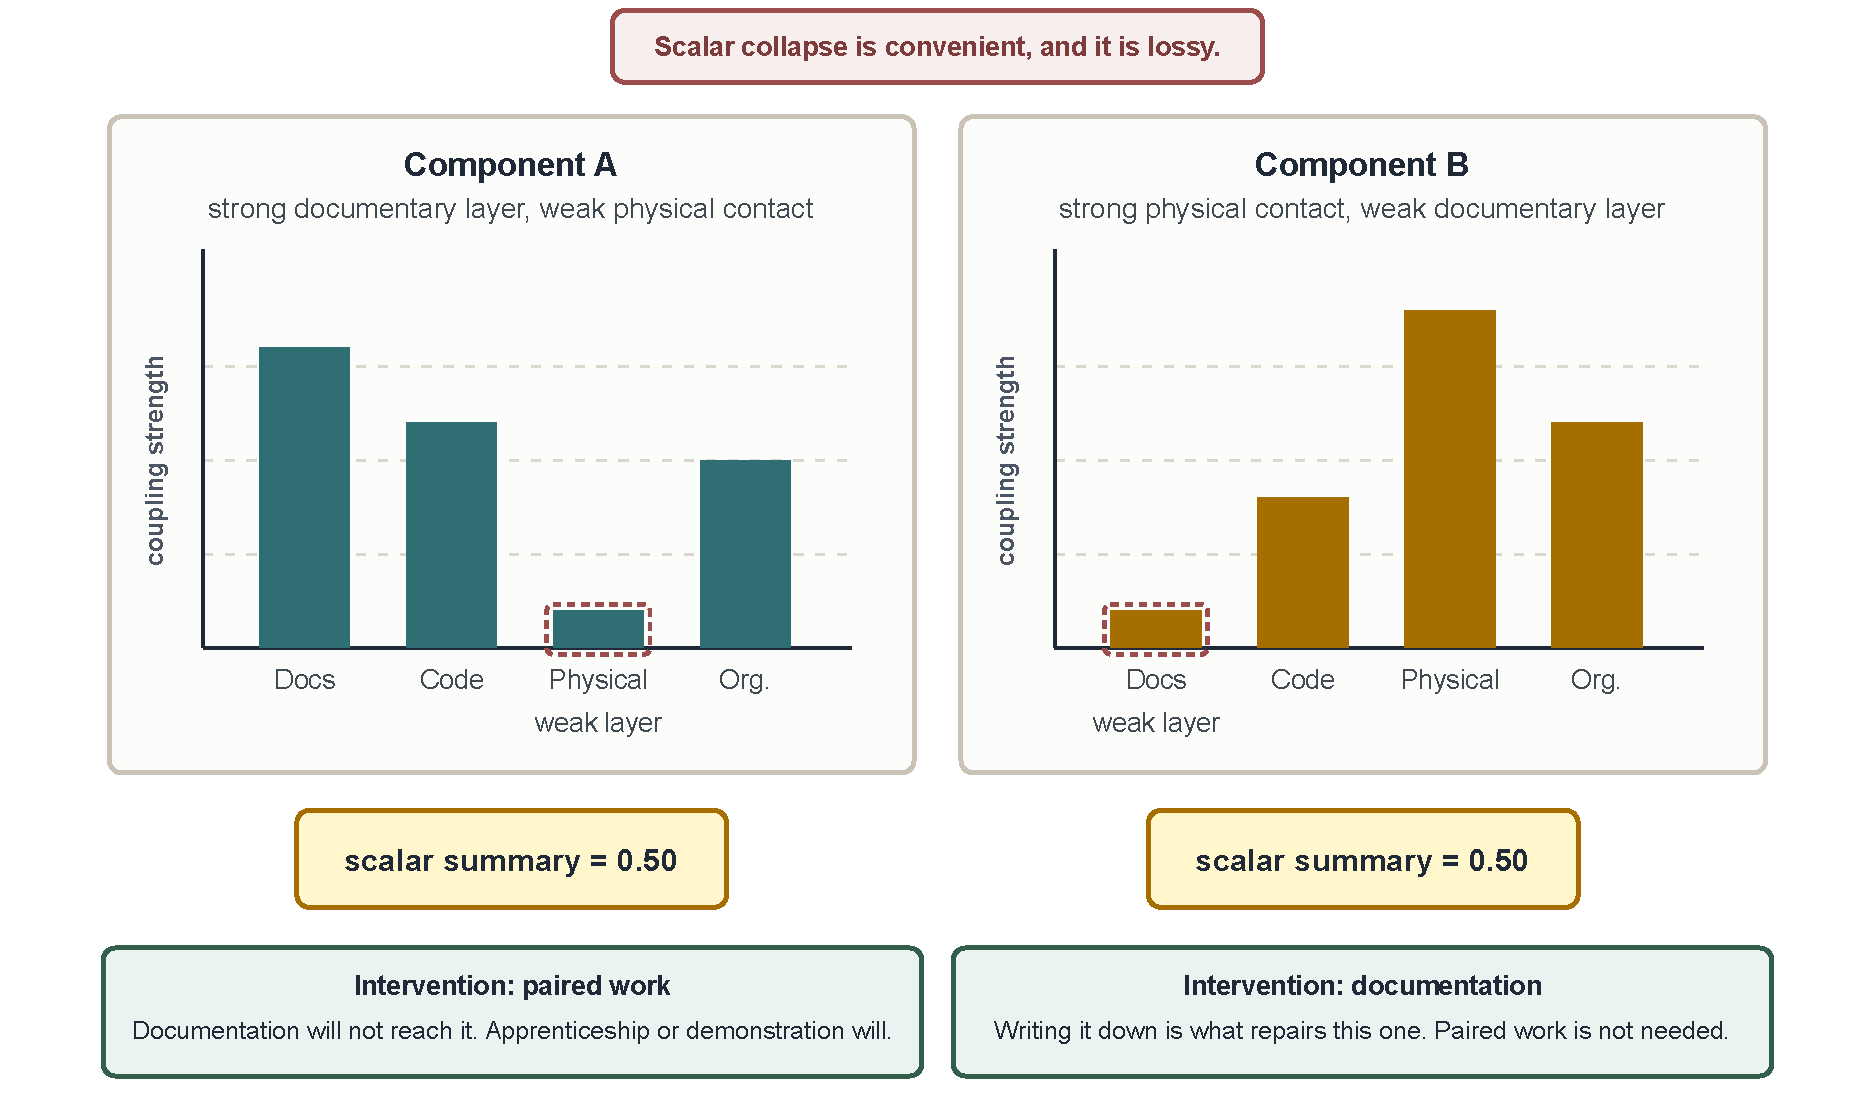
\includegraphics[width=0.86\textwidth]{fig3_gradient_stays_a_vector_print.pdf}
\caption{Two components with the same scalar summary and different layer profiles. Component A has a strong documentary layer and weak physical contact; Component B is the reverse. Both reduce to 0.50. The intervention that repairs one will not reach the other, which is why coupling strength is recorded per layer rather than as a single value.}
\label{fig:gradient-vector}
\end{figure*}


\section{Current-Stage Evaluation}\label{sec:9}

Uses of the map and validation of those uses are separate questions. Verified records make query, comparison, layer profiles, and later repeated collection possible, but they do not by themselves establish that the resulting measures are valid or predictive. At the present collection stage, the first evaluation question is whether records can be produced in a form stable enough to accumulate.

Success at this stage concerns the form of the records rather than the values inside them. Fields that work with variable observations, including clinical trials, epidemiology, and satellite measurement, do not begin by assuming every observation will agree. They begin by making the collection procedure explicit enough that variation can be interpreted. IAKM requires the same kind of discipline. A record must be locatable, source-traceable, convention-bound, and auditable. Collections must be poolable across analysts, systems, and domains, because records that cannot join other records cannot form a corpus. Fig.~\ref{fig:collection-stage} pairs each of those criteria with the collection failure it prevents, and separates the standards work that follows from the science that depends on it.

A corpus is a collection of records produced under declared conventions so that they can be pooled, compared, audited, and analyzed together. The necessary conventions include how fields and domains are named, how layers are derived, how evidence is admitted, how missingness is recorded, how reviewer standing is defined, how disagreements are reconciled, how addresses are versioned, and how coupling strength or later scalar reductions are calibrated. If those choices remain implicit, independently produced maps become separate descriptions rather than cumulative evidence. If they are fixed too early and without versioning, the wrong categories are encoded at scale.

The basic observation can still be simple. For a declared address, a record either verifies that a knowledge-relevant relation was observed or it does not. Many yes-or-no observations can later support probabilistic claims about where knowledge-relevant metadata tends to appear and which interface conditions change those probabilities. The methodology therefore requires stable records, not deterministic claims that a type of interface always contains a type of knowledge.

The checks available at this stage ask whether the collection procedure produces records stable, interpretable, and varied enough to justify further study. Table~\ref{tab:checks} states those checks.

\begin{table*}[!b]
\caption{Collection-stage checks, and what would support continuing.}
\label{tab:checks}
\centering
\scriptsize
\begin{tabularx}{\textwidth}{W{0.65}W{1.35}}
\hline
\textbf{Collection-stage question} & \textbf{What would support continuing} \\
\hline
Can addresses be located reproducibly? & Analysts using the same sources and declared field-domain lens locate substantially similar addresses \\
Can records be verified consistently? & Reviewers with standing make comparable disposition decisions on the same candidate records \\
Can the record structure preserve uncertainty? & Unknowns are recorded explicitly rather than hidden as blanks \\
Do layer profiles vary? & Components differ by layer profile, showing that the vector carries information a single value would discard \\
Do single-knower dependencies surface recognizably? & Components named by the map as having one associated knower are recognized by participants as difficult to recover \\
Does declaring a binding do any work? & Some addresses are locatable only under the declared field-domain lens, showing that the binding changes what the map can see \\
\hline
\end{tabularx}
\end{table*}

These checks do not validate prediction, intervention, or generalizability. They ask whether the collection procedure produces records stable and varied enough to support the next stage of study; a negative answer is a reason to revise the procedure before collecting further.

A precedent exists for the last check. Truck factor estimates computed from repository history were taken back to the developers of the systems they described. In eighty-four percent of valid answers, developers agreed or partially agreed that the identified developers were the main authors of their systems, while fifty-three percent gave a positive or partially positive response about the estimated truck factor itself \cite{avelino2016}. The same distinction matters here. Who is connected to a component is a claim people can often confirm from where they sit; the value attached to that connection requires more evidence.

Until these checks are run, IAKM should be claimed as a digital mapping system with a coordinate system and methodology for producing verified records, not as a validated predictor of loss. Section~\ref{sec:10} turns from collection-stage checks to the standards and longitudinal work needed next.


\begin{figure*}[!t]
\centering
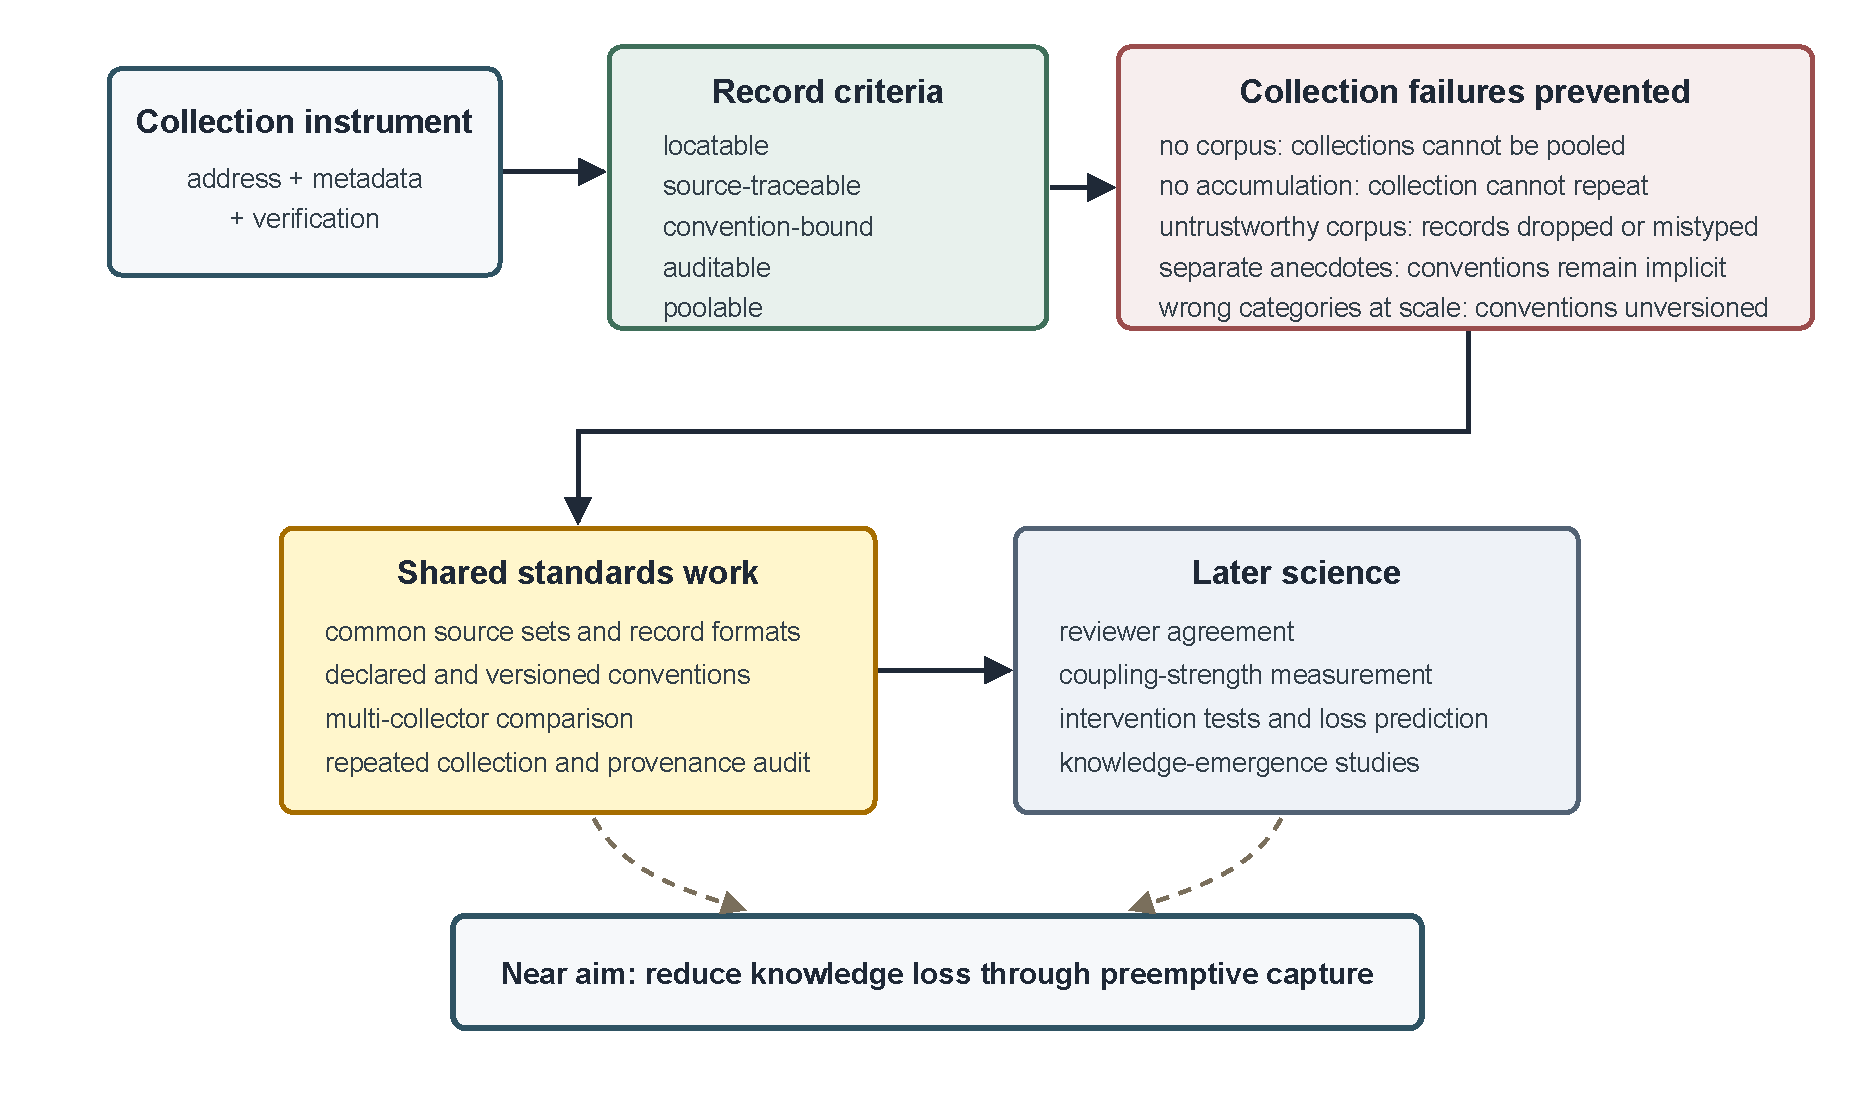
\includegraphics[width=0.86\textwidth]{fig4_collection_stage_print.pdf}
\caption{The collection stage. Each record criterion prevents a specific collection failure. Shared standards work follows from the collection instrument; the science that depends on a corpus, including reviewer agreement, coupling-strength measurement, intervention tests, and knowledge-emergence studies, follows from that. The near aim is reduction of knowledge loss through preemptive capture.}
\label{fig:collection-stage}
\end{figure*}


\section{Standards and Future Work}\label{sec:10}

Mature sciences make variation studyable by standardizing how observations are named, measured, and reported. Chemistry has shared naming conventions and reporting standards. Physics has agreed units and calibration practices. Those conventions do not remove variation from the world; they make observations comparable despite variation. IAKM is at an earlier stage.

The next stage for the field is standards-building through shared collection. IAKM can specify a record form, coordinate system, and verification procedure, but cumulative study requires conventions that no single author can settle alone. Fields and domains have to be bounded, layers have to be derived, evidence rules have to be declared, reviewer standing has to be defined, and record formats have to be stable enough for separate collections to join.

That work requires other collectors because the central claims concern reproducibility, comparability, and accumulation. A record reproduced only by the person who produced it has not yet been reproduced. Nor can agreement be assumed: in one many-analyst study, twenty-nine teams working from the same dataset and question reached materially different conclusions, with sixty-nine percent finding a significant effect and thirty-one percent not, and neither analyst expertise nor peer-rated quality readily explained the variation \cite{silberzahn2018}. The deployment reported above also makes the need for shared collection concrete: it used one binding, reached two of five exposed layers, drew on one program's sources, and was checked by one person against a sample.

Other fields already have methods for building conventions when categories are still emerging. The relevant question is which method family can help build which part of an IAKM collection standard. Table~\ref{tab:families} names the candidate families.

\begin{table*}[!tb]
\caption{Method families that build conventions in emerging fields.}
\label{tab:families}
\centering
\scriptsize
\begin{tabularx}{\textwidth}{XXX}
\hline
\textbf{Method family} & \textbf{Where it is established} & \textbf{What it can help build for IAKM} \\
\hline
Delphi studies & Expert consensus and standards development; Dalkey and Helmer [12] & Convergence on definitions, categories, reviewer rules, and convention choices \\
Evaluation campaigns and shared tasks & Ontology matching, OAEI; shared tasks in natural language processing and information retrieval & Shared source sets, common output formats, benchmark comparison, visible disagreement \\
Reference corpus construction & Corpus linguistics and information retrieval evaluation; Biber [13] & Common records built under documented sampling and annotation rules \\
Registry design & Medical and public health registries; AHRQ registry user guide & Stable schemas, longitudinal accumulation, versioned data definitions \\
Systematic review protocols & Evidence synthesis; PRISMA & Inclusion criteria, extraction fields, source traceability, disagreement handling \\
Content analysis and codebook development & Communication research and qualitative methods & Coding rules, coder training, agreement checks, category refinement \\
Ontology engineering & Knowledge representation; METHONTOLOGY & Formal vocabulary, classes, relations, identity rules \\
Many-analyst designs & Metascience; Silberzahn et al. [11] & Shows where competent analysts diverge under shared data and task definitions \\
Measurement-instrument development & Psychometrics; COSMIN & Reliability, validity, calibration, construct definition \\
Records and provenance standards & Archival records management; ISO 15489 & Provenance, audit trails, record metadata, custody, traceability \\
\hline
\end{tabularx}
\end{table*}

Shared collection studies would test whether different analysts and reviewers can produce compatible records from common source sets. Those studies would show where the current methodology is reproducible and where conventions need to be written, narrowed, or versioned.

These methods are not adopted here as a fixed procedure. They identify the kinds of standards work needed before IAKM collections can accumulate into a corpus.

With future funding and access, the next study would continue the CubeSat work as a baseline while developing comparable mapping systems in other domains alongside it. Continued CubeSat collection would allow verified records to be compared with changes in the organization, changes in components, data collected through ground stations, and operational outcomes after launch. New domains would test how the methodology changes when the mapped system, evidence sources, components, and outcomes differ.

The goal would not be to compare domains as if they should produce the same records. It would be to learn which models, components, sources, and levels of granularity make different outcomes more interpretable, as shown in Fig.~\ref{fig:future-work}.


\begin{figure*}[!tb]
\centering
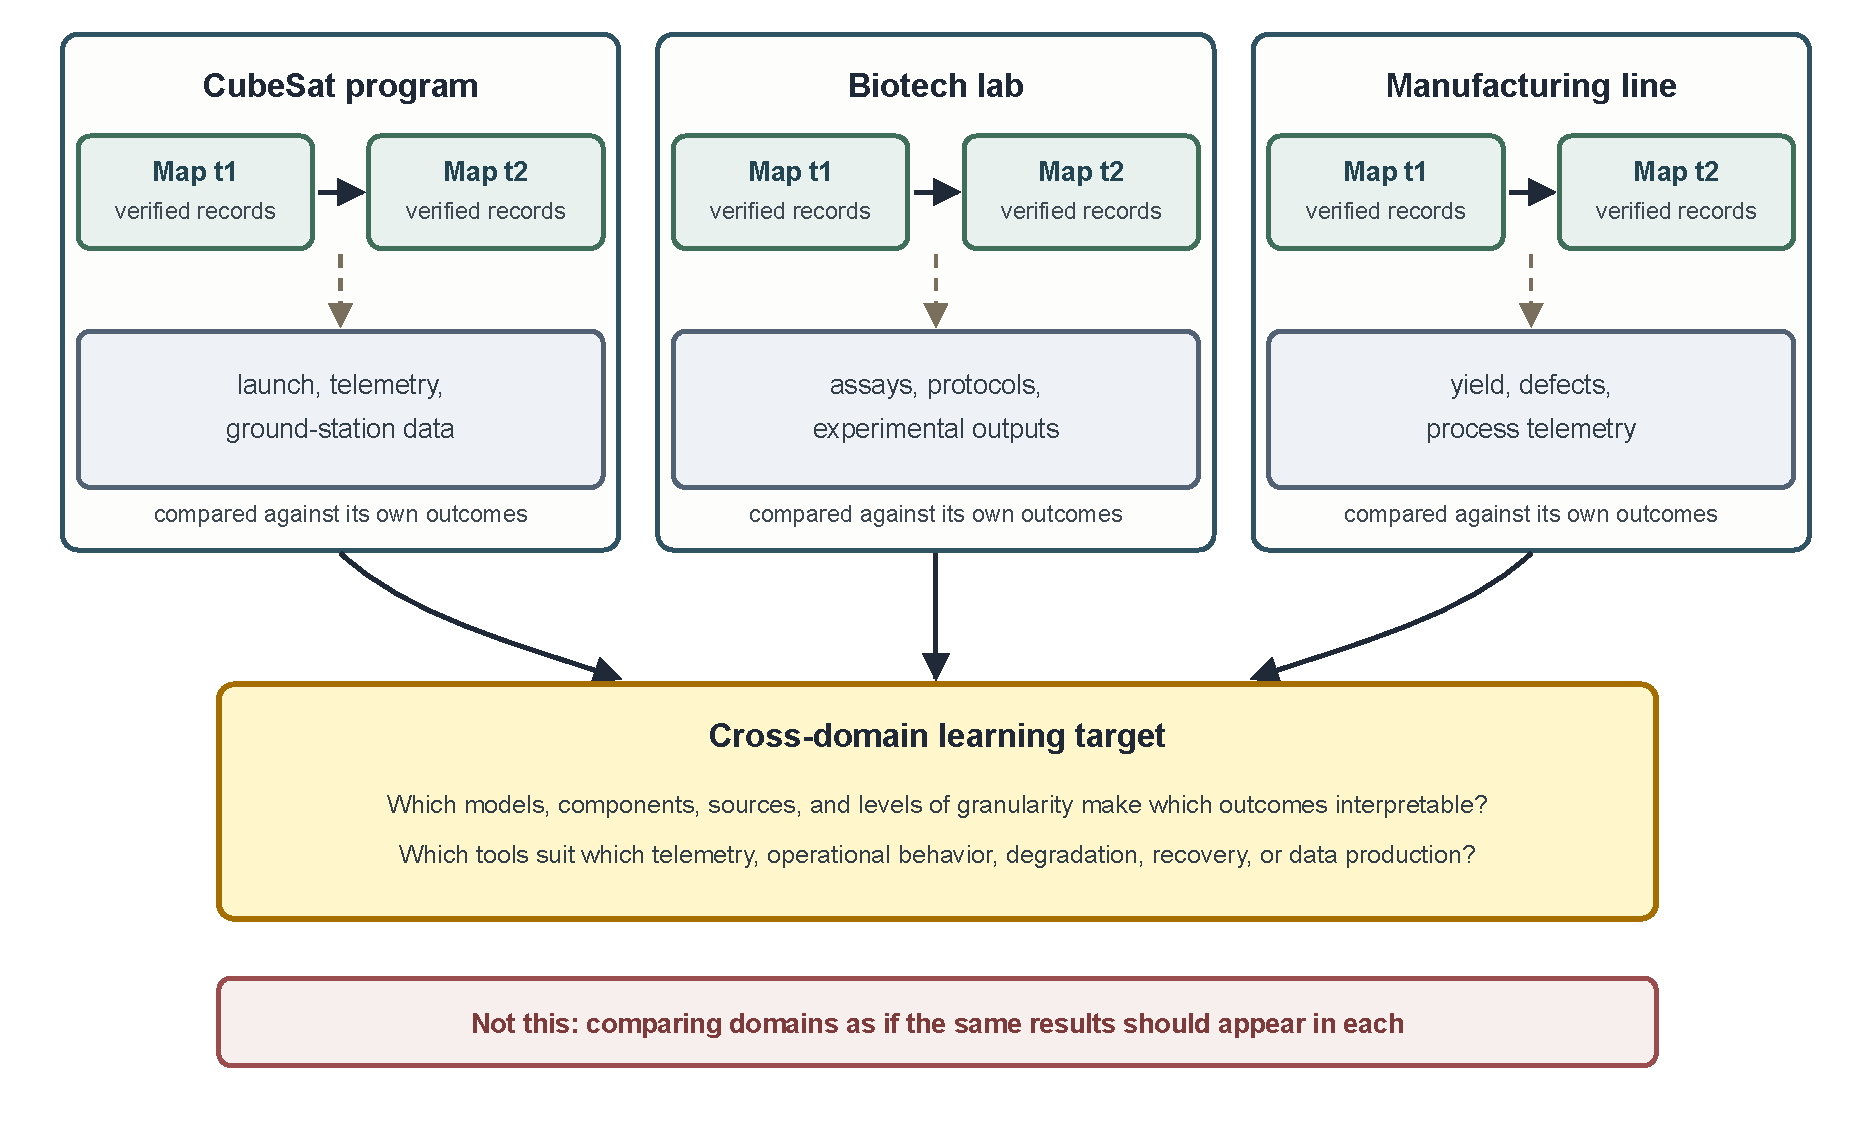
\includegraphics[width=0.78\textwidth]{fig5_future_work_print.pdf}
\caption{Cross-domain future work. Each domain is mapped at two times and compared against its own outcomes, not against the other domains. The learning target is which models, components, sources, and levels of granularity make which outcomes interpretable.}
\label{fig:future-work}
\end{figure*}
 Different domains may require different surfaces, component models, and outcome measures. Keeping the CubeSat work as a baseline while building new domain maps would show what remains stable in the methodology and what must be adapted.

Repeated collection may also support later study of knowledge emergence. If comparable interface relations recur where new knowledge forms, then interface identification may help researchers know where to look while knowledge is still forming. That possibility requires a longitudinal corpus and shared conventions; it is future work, not a claim established here.

\section{Conclusion}\label{sec:11}

IAKM is a collection-stage mapping system. It addresses knowledge loss by making knowledge-relevant metadata structurally addressable before recovery becomes impossible, and its present contribution is a coordinate system, a collection convention, and a verification procedure.

AI-assisted analysis creates the observational opportunity, because large artifact sets can be examined while work is still ongoing and candidate interface relations can be identified before the people, practices, and traces that carry recoverable knowledge disappear. IAKM supplies the constraint that makes those observations scientific rather than merely extensive.

What the methodology does not yet establish is a validated predictor of loss, a calibrated measure of coupling strength, or an intervention model. Each requires a corpus, and a corpus requires shared standards, repeated collection, and validation by parties other than the author.

The longer horizon, set out in Section~\ref{sec:10}, is whether the same records can support the study of knowledge emergence.

Knowledge loss in modular sociotechnical systems cannot become a cumulative science until knowledge-relevant metadata is collected under shared, auditable, versioned conventions. IAKM is a proposed digital mapping system and methodology for making that work possible.


\begin{thebibliography}{99}

\bibitem{simon1962} H. A. Simon, ``The architecture of complexity,'' \emph{Proc. Amer. Philos. Soc.}, vol. 106, no. 6, pp. 467--482, Dec. 12, 1962.

\bibitem{pimmler1994} T. U. Pimmler and S. D. Eppinger, ``Integration analysis of product decompositions,'' in \emph{Proc. ASME 1994 Design Technical Conf., 6th Int. Conf. Design Theory and Methodology}, Minneapolis, MN, USA, Sept. 11--14, 1994, pp. 343--351, doi: 10.1115/DETC1994-0034.

\bibitem{browning2016} T. R. Browning, ``Design structure matrix extensions and innovations: A survey and new opportunities,'' \emph{IEEE Trans. Eng. Manage.}, vol. 63, no. 1, pp. 27--52, Feb. 2016, doi: 10.1109/TEM.2015.2491283.

\bibitem{argote1999} L. Argote, \emph{Organizational Learning: Creating, Retaining and Transferring Knowledge}. Boston, MA, USA: Kluwer Academic, 1999.

\bibitem{galan2023} N. Galan, ``Knowledge loss induced by organizational member turnover: A review of empirical literature, synthesis and future research directions (Part I),'' \emph{Learn. Organ.}, vol. 30, no. 2, pp. 117--136, 2023, doi: 10.1108/TLO-09-2022-0107.

\bibitem{lave1991} J. Lave and E. Wenger, \emph{Situated Learning: Legitimate Peripheral Participation}. Cambridge, U.K.: Cambridge Univ. Press, 1991, doi: 10.1017/CBO9780511815355.

\bibitem{hutchins1995} E. Hutchins, \emph{Cognition in the Wild}. Cambridge, MA, USA: MIT Press, 1995, doi: 10.7551/mitpress/1881.001.0001.

\bibitem{hjorland1995} B. Hj{\o}rland and H. Albrechtsen, ``Toward a new horizon in information science: Domain-analysis,'' \emph{J. Amer. Soc. Inf. Sci.}, vol. 46, no. 6, pp. 400--425, 1995, doi: 10.1002/(SICI)1097-4571(199507)46:6\textless{}400::AID-ASI2\textgreater{}3.0.CO;2-Y.

\bibitem{hjorland2002} B. Hj{\o}rland, ``Domain analysis in information science: Eleven approaches --- traditional as well as innovative,'' \emph{J. Documentation}, vol. 58, no. 4, pp. 422--462, 2002, doi: 10.1108/00220410210431136.

\bibitem{avelino2016} G. Avelino, L. Passos, A. Hora, and M. T. Valente, ``A novel approach for estimating Truck Factors,'' in \emph{Proc. 2016 IEEE 24th Int. Conf. Program Comprehension (ICPC)}, Austin, TX, USA, 2016, pp. 1--10, doi: 10.1109/ICPC.2016.7503718.

\bibitem{silberzahn2018} R. Silberzahn, E. L. Uhlmann, D. P. Martin, \emph{et al.}, ``Many analysts, one data set: Making transparent how variations in analytic choices affect results,'' \emph{Adv. Methods Practices Psychol. Sci.}, vol. 1, no. 3, pp. 337--356, 2018, doi: 10.1177/2515245917747646.

\end{thebibliography}

\end{document}
